\documentclass[notitlepage]{report}

\title{
	\textsc{ \small
		Physics 415
	} \\
	{\textsc{\small Lab \#6}} \\
	Electron Beam Diffraction/Debye-Scherrer Diffraction at Graphite
}
\author{Kevin Evans \\ Partner: Sierra Ray}
\date{April 8, 2021}
\usepackage{amssymb}
\usepackage{mathtools}
\usepackage{import}
\usepackage{color}
\usepackage{amsthm}
\usepackage{amsmath}
\usepackage{slashed}
\usepackage{relsize}
\usepackage{threeparttable}
\usepackage{float}
\usepackage{booktabs}
\usepackage{boldline}
\usepackage{changepage}
\usepackage{physics}
\usepackage[inter-unit-product =\cdot]{siunitx}
\usepackage{setspace}
\usepackage{caption}
\usepackage{subcaption}
\usepackage[makeroom]{cancel}
%\usepackage{pgfplots}

\usepackage{enumitem}
\usepackage{times}
\usepackage{titling} % for titlingpage environment
\usepackage{calligra}
\usepackage{graphicx}
\DeclareMathAlphabet{\mathcalligra}{T1}{calligra}{m}{n}
\DeclareFontShape{T1}{calligra}{m}{n}{<->s*[2.2]callig15}{}
\newcommand{\scriptr}{\mathcalligra{r}\,}
\newcommand{\boldscriptr}{\pmb{\mathcalligra{r}}\,}
\newcommand{\emf}{\mathcal{E}}
\renewcommand{\thesection}{\arabic{section}}

\begin{document}
	\begin{titlingpage}
		\maketitle
		\begin{abstract}
			\noindent In a short series of experiments, electron diffraction patterns of graphite powder was observed. Using a heated cathode ray, electrons were diffracted against graphite powder and projected onto a phosphor screen. The diffraction rings were then compared against the expected value using the Bragg equation. 
			The carbon lattice was found to have an average lattice spacing $d=\SI{1.693}{\angstrom}$. Relative to an accepted value of \SI{1.42}{\angstrom}, this led to 19\% error. Connecting the anode and focusing electrode to \SI{2.5}{\kV} leads to a large image being formed on the screen, likely due to the focusing electrode now acting as a divergent lens.
		\end{abstract}
	\end{titlingpage}

	\section{Description of Experiment}
	
	All particles have a wavelength given by the de Broglie wavelength, \begin{equation}
		\lambda  = h / p. \label{eq:deBroglie}
	\end{equation}
	Additionally, diffraction off crystal lattices can be described using Bragg scattering. Under the condition where the wavelength is comparable to the lattice spacing, i.e. the atomic spacing, specular reflection can occur and interfere with different levels of the lattice. From Figure \ref{fig:braggplanediffraction}, constructive interference can be shown to obey the condition \begin{equation}
		2d \sin \theta = n \lambda \label{eq:bragg}
	\end{equation}
	where $d$ is the regular lattice spacing, $n$ is the order ($n=1, 2, 3,\dots$), $\lambda$ is the wavelength of the incident wave, and $\theta$ denotes the angle of reflection relative to the lattice plane.

	\begin{figure}[h]
		\centering
		 \def\svgwidth{0.6\linewidth}
		\input{BraggPlaneDiffraction.pdf_tex}
		\caption{Bragg diffraction off the first two planes of a crystal lattice (Wikipedia).}
		\label{fig:braggplanediffraction}
	\end{figure}
	
	In this experiment, a graphite powder was used instead of a single crystal. The incident electron beam encounters random orientations of the crystal, leading to the electron beam scattering into concentric diffraction rings. The heated cathode ray tube was brought to a bias voltage of \SI{5}{\kV}. The experimental setup is shown in Figure \ref{fig:expsetup} below. Reducing the voltage to \SI{3}{\kV} and \SI{4}{\kV} creates a larger diffraction pattern on the phosphor screen. The pattern was sketched in the lab notebook and the ring spacings were noted.
	
	Next, the anode and focusing electrode were connected to \SI{2.5}{\kV}, leaving the cathode at ground. The projected image on the phosphor was sketched in the lab notebook.
	\begin{figure}[p]
		\centering
		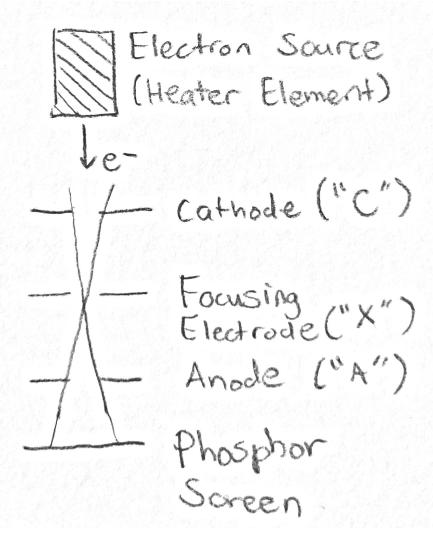
\includegraphics[width=0.5\linewidth]{expsetup}
		\caption{Diagram of the experimental setup.}
		\label{fig:expsetup}
	\end{figure}
	
	\section{Data and Analysis}
	After setting the acceleration voltage to \SI{5}{\kV}, the diameters of the diffraction rings were recorded in Table \ref{table:lattice}. The average spacing is \SI{1.693}{\angstrom}. The accepted value of the average spacing in graphite is \SI{1.42}{\angstrom}. This leads to roughly 19\% error.
	
	\begin{table}[h]
		\centering
		\caption{Measured diameters and corresponding calculated lattice spacing.}
		\label{table:lattice}
		\begin{tabular}{ccc}
			\toprule
			$n$ & Diameter [\si{cm}] & Spacing $d$ [\si{\m}] \\
			\midrule
			$3$ & \num{4.3} & \num{1.65e-10} \\
			$2$ & \num{2.4} & \num{1.96e-10} \\
			$1$ & \num{1.6} & \num{1.47e-10} \\
			\bottomrule
		\end{tabular}
	\end{table}

	After connecting the anode and focusing electrode together at \SI{2.5}{\kV}, an image of the approximate shape of the beam path formed on the screen with no diffraction pattern appearing.
	
	This is likely due to the electrode now being attractive for the electron beam. Previously, the focusing electrode repulsed the electron beam, creating a convergent beam. This is analogous to classical optics: now, the focusing electrode acts as a divergent lens and before, it would act as a convergent (focusing) lens.
	

	\begin{figure*}[p]
		\centering
		\begin{subfigure}[t]{0.5\textwidth}
			\centering
			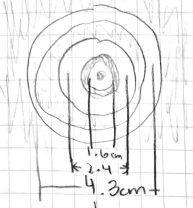
\includegraphics[height=1.4in]{init}
			\caption{Initial experiment setup}
		\end{subfigure}%
		~ 
		\begin{subfigure}[t]{0.5\textwidth}
			\centering
			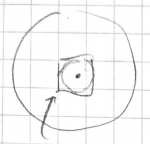
\includegraphics[height=1.2in]{divergent}
			\caption{Anode and focusing electrode at \SI{2.5}{\kV}.}
		\end{subfigure}
		\caption{Rough sketches of the images on the phosphor screen.}
	\end{figure*}
	\section{Results and Conclusion}
	The carbon lattice was found to have an average lattice spacing $d=\SI{1.693}{\angstrom}$. Relative to an accepted value of \SI{1.42}{\angstrom}, this led to 19\% error. Connecting the anode and focusing electrode to \SI{2.5}{\kV} leads to a large image being formed on the screen, likely due to the focusing electrode now acting as a divergent lens.
	
	\pagebreak
	\section{Worksheet Problems} 
	\begin{enumerate}
		\item[(a)] The spacing can be determined using eq. (6), \begin{align*}
			d & = \frac{n \lambda}{2 \sin \theta} \\
				& = \frac{\SI{1.5420}{\angstrom}}{2 \sin 50^\circ} = \SI{2.15}{\angstrom}
		\end{align*}
	
		\item[(b)] The wavelength can be found using \begin{align*}
			\lambda & = d \sin \theta \\
				& = \SI{2.15}{\angstrom} \times \sin 50^\circ = \SI{1.647}{\angstrom}
			\intertext{Using the de Broglie relationship,}
			\lambda& = \frac{h}{\sqrt{2 mE}} \\
				& = \frac{\SI{1.2398}{\eV \um}}{\sqrt{2 \times (\SI{0.511}{\MeV}) \times (\SI{54}{\eV})}} \\
				& = \SI{1.669}{\angstrom}
		\end{align*}
		These two wavelengths are about equal.
		
		\item[(c)] Using the two given equations, \begin{align*}
			h / mv & = 2 \times \SI{1.5e-8}{\centi\meter} \times \sin(30^\circ) \\
			v & = \SI{2661}{\m\per\s}
		\end{align*}
	
		\item[(d)] Solving for the temperature $T$, \begin{align*}
			T & = \frac{2}{3 k} \times \frac{1}{2} mv^2 \\
				& = \frac{2}{6 \times \SI{1.381e-23}{J \per \K}} \times \SI{1.66e-24}{\g} \times \left(\SI{2661}{\m\per\s}\right)^2 \\
				& = \SI{283.7}{\K}
		\end{align*}
	\end{enumerate}
	\section*{Lab notebook}
\begin{center}
	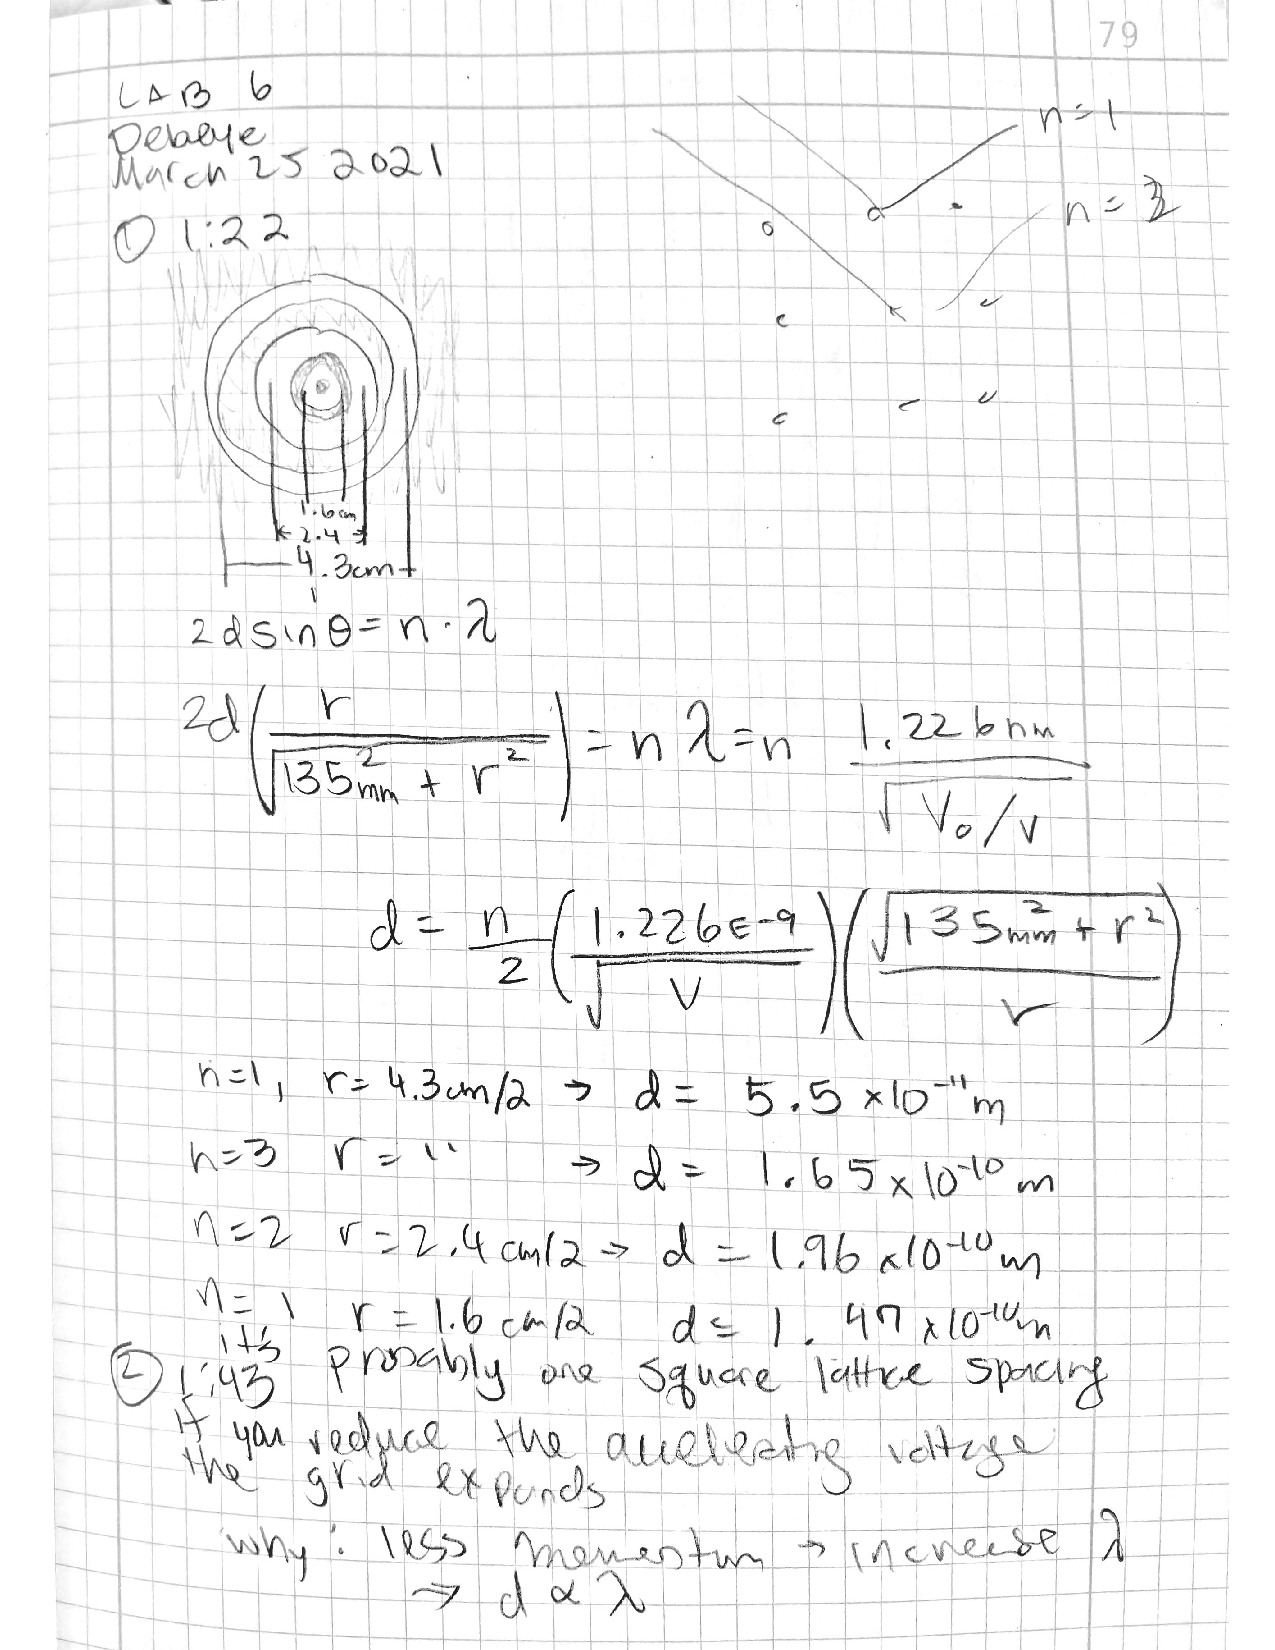
\includegraphics[width=\linewidth,page=1,clip]{Scanned_20210406-1310}
\end{center}
\begin{center}
		\includegraphics[width=\linewidth,page=2,clip]{Scanned_20210406-1310}
\end{center}
\end{document}